\documentclass[]{manual}

\title{Diffraction}
\date{\today}
\course{Physics 325}

\begin{document}
    \maketitle
    \thispagestyle{firstpage}

    %%%

    \section{Motivation}
    
    One of the primary concerns in optics is the measurement and manipulation of the properties of light itself.
    Even other experiments that simply use light to perform some other task typically need to begin by creating that light in the first place.
    The best (and one of the only) ways of measuring the microscopic properties of light - wavelength and frequency - is to exploit that fact that light can \emph{interfere} with itself.
    In this lab we will investigate \emph{diffraction}, a common and useful interference phenomenon.


    \section{Background}
    
    The \emph{superposition principle} of electromagnetism tells us that electric fields can be added to each other as long as they both obey Maxwell's equations independently.
    So, if we have two one-dimensional electric fields, $E_1(x, t)$ and $E_2(x, t)$, the total electric field would be
    \begin{align} \label{eqn:electric-field-superposition}
        E(x, t) = E_1(x, t) + E_2(x, t).
    \end{align}
    Suppose these electric fields belong to a propagating electromagnetic wave (i.e., light) and are shone on a screen.
    What do we expect to see on the screen?
    
    What we see depends on the \emph{intensity} of the light, which is proportional to the square of the electric field:
    \begin{align} \label{eqn:electric-field-intensity-with-time-dependence}
        I(x, t) &= \epsilon_0 c \, E^2(x, t) \nonumber \\
        I(x, t) &= \epsilon_0 c \,  \qty[ E_1^2(x, t) + E_2^2(x, t) + E_1(x, t) E_2(x, t) ]
    \end{align}
    Equation~\eqref{eqn:electric-field-intensity} is appropriate in a vacuum, where $\epsilon_0$ is the vacuum permittivity and $c$ is the speed of light.
    The first two terms are what we would expect from the intensity of the individual fields.
    The last term is the \emph{interference}: it depends on the product of the electric fields, so it could be positive or negative or zero at any given point.
    Because these electric field oscillate very quickly, there's a lot of interference going on that we won't actually see.
    To find out what the human eye would actually see, we average over time, assuming that each electric field oscillates sinusoidally in time:
    Then we have
    \begin{align} \label{eqn:electric-field-intensity}
        I(x) &= \frac{1}{2} \epsilon_0 c \,  \qty[ E_1^2(x) + E_2^2(x) + E_1(x) E_2(x) ].
    \end{align}
    
    The above analysis is good for our intuition, but doesn't reflect a real physical system.
    In this lab we will investigate one of the most common interference phenomena: \emph{diffraction}.
    Diffraction occurs when light is forced to travel through an aperture.
    The first aperture we will consider is a \emph{slit}, a rectangular hole in an otherwise-opaque barrier.
    The situation is illustrated in Figure~\ref{fig:single-slit-diffraction-geometry}.
    
    \begin{figure}
        \centering
        
        \begin{tikzpicture}
            \draw[rounded corners] (-3,5) -- (-2.8,4.5) -- (-2.9,4) -- (-2.5,3.5) -- (-2.7,3) -- (-2.4,2.5) -- (-2.6,2) -- (-2.5,1.5) -- (-2.9,1) -- (-2.7,0.5) -- (-3,0);
            \draw[rounded corners] (-2.6,5) -- (-2.4,4.5) -- (-2.5,4) -- (-2.1,3.5) -- (-2.3,3) -- (-2.0,2.5) -- (-2.2,2) -- (-2.1,1.5) -- (-2.5,1) -- (-2.3,0.5) -- (-2.6,0);
            \draw[rounded corners] (-2.2,5) -- (-2.0,4.5) -- (-2.1,4) -- (-1.7,3.5) -- (-1.9,3) -- (-1.6,2.5) -- (-1.8,2) -- (-1.7,1.5) -- (-2.1,1) -- (-1.9,0.5) -- (-2.2,0);
            
            \draw[|<->|, dashed] (-0.3,2) -- (-0.3,3) node[midway, left] {$W$};
            
            \draw[ultra thick] (0,0) -- (0,2);
            \draw[ultra thick] (0,3) -- (0,5) node[above] {Barrier w/ Slit};
            
            \draw[dashed] (0,2.5) -- (9,2.5) node[midway, below] {$L$};
            
            \draw[dashed] (0,2.5) -- (9,3.5) node[midway, above] {$r$};
            
            \draw[|<->|, dashed] (9.2,2.5) -- (9.2,3.5) node[midway, right] {$x$} node[above right] {Observation Point};
            
            \draw[<->, dashed] (7,2.5) arc (0:6.4:7) node[midway, right] {$\theta$};
            
            \draw[fill] (0,2.5) circle [radius=0.05];
            \draw (0,2.5) -- (0.5,2.25);
            \node[align=center,below] at (1,2.35) {$(z_0, \, 0)$};
            
            \draw[fill] (0,2.75) circle [radius=0.05];
            \draw (0,2.75) -- (0.5,2.85);
            \node[align=center,above] at (1,2.7) {$(z_0, \, w)$};
            
            \draw (9, 0) -- (9, 5) node[above] {Screen};
            
            \draw[fill] (9,3.5) circle [radius=0.05];
        \end{tikzpicture}
        
        \caption{An electromagnetic wave illuminating a single slit.}
        
        \label{fig:single-slit-diffraction-geometry}
    \end{figure}
    
    To determine what we see on the screen (i.e., $I(x)$), we will use \emph{Huygen's Principle}, which says that we can treat each point in the plane of the rectangular hole as an independent spherical emitter.
    To determine the electric field anywhere, we just sum over the contributions from each point (after making some approximations which we won't describe in detail here):
    \begin{align}
        E(z, x) &= \int^{W/2}_{-W/2} \dd{w} E(z_0, w) \, \frac{e^{i k r}}{r},
    \end{align}
    where $z$ is the coordinate going between the barrier and the screen, $x$ is the distance along the screen to the observed point, $r$ is the distance from the center of the slit to the observed point on the screen, $k = 2 \pi / \lambda$ is the wavenumber of the light, and $W$ is the width of the slit.
    The integration variable $w$ tracks where the integral is along the slit.
    The field on the screen is
    \begin{align}
        E(x) &= \int^{W/2}_{-W/2} \dd{w} E(z_0, w) \, \frac{e^{i k \sqrt{(w-x)^2 + L^2}}}{\sqrt{(w-x)^2 + L^2}}.
    \end{align}
    
    This integral is not tractable without making some assumptions.
    We will assume that we are in the \emph{far-field}: $L \gg W$.
    This type of diffraction is called \emph{Fraunhofer diffraction}.
    We can now approximate the square root in the exponent as
    \begin{align}
        \sqrt{(s-x)^2 + L^2} = \sqrt{w^2 + x^2 - 2wx + L^2} = r \, \sqrt{1 + \frac{-2wx + w^2}{r^2}} \approx r \qty(1 - \frac{wx}{r^2}),
    \end{align}
    and the square root in the denominator as $\sqrt{(w-x)^2 + L^2} \approx r$.
    Now we have
    \begin{align}
        E(x) &= \frac{e^{i k r}}{r} \, \int^{W/2}_{-W/2} \dd{w} E(z_0, w) \, e^{-i k \frac{x}{r} w},
    \end{align}
    so we've managed to pull out an overall prefactor that means that the integral itself only accounts for deviations from the pattern produced by a point source at the center of the slit.
    Suppose that the incoming electromagnetic wave is a plane wave, so that $E(z_0, w) = E_0$.
    Then
    \begin{align} \label{eqn:single-slit-diffraction-field}
        E(x) &= E_0 \, \frac{e^{i k r}}{r} \, \int^{W/2}_{-W/2} \dd{w} e^{-i k \frac{x}{r} w} \nonumber \\
        E(x) &= E_0 \, W \, \frac{e^{i k r}}{r} \sinc\qty(\pi \, \frac{W}{\lambda r} \, x),
    \end{align}
    where $\sinc(x) \equiv \sin(x) / x$, and $\sinc(0) = 1$.
    Since we're working with complex field amplitudes, the resulting intensity is
    \begin{align} \label{eqn:single-slit-diffraction-intensity}
        I(x) = E(x) \, E^*(x) = \frac{E_0^2 \, W^2}{r^2} \sinc^2\qty(\pi \, \frac{W}{\lambda r} \, x).
    \end{align}
    This intensity profile is shown in Figure~\ref{fig:single-slit-diffraction-intensity}.
    The zeros of $\sinc^2(y)$ occur at $y = 0, \pi, 2 \pi, 3 \pi, \cdots$.
    The positions of the maxima are not evenly spaced and must be calculated numerically.
    The first few are tabulated to a few digits of precision in Table \ref{tab:sinc-squared-maxima}.
    
    \begin{figure}
        \centering
        
        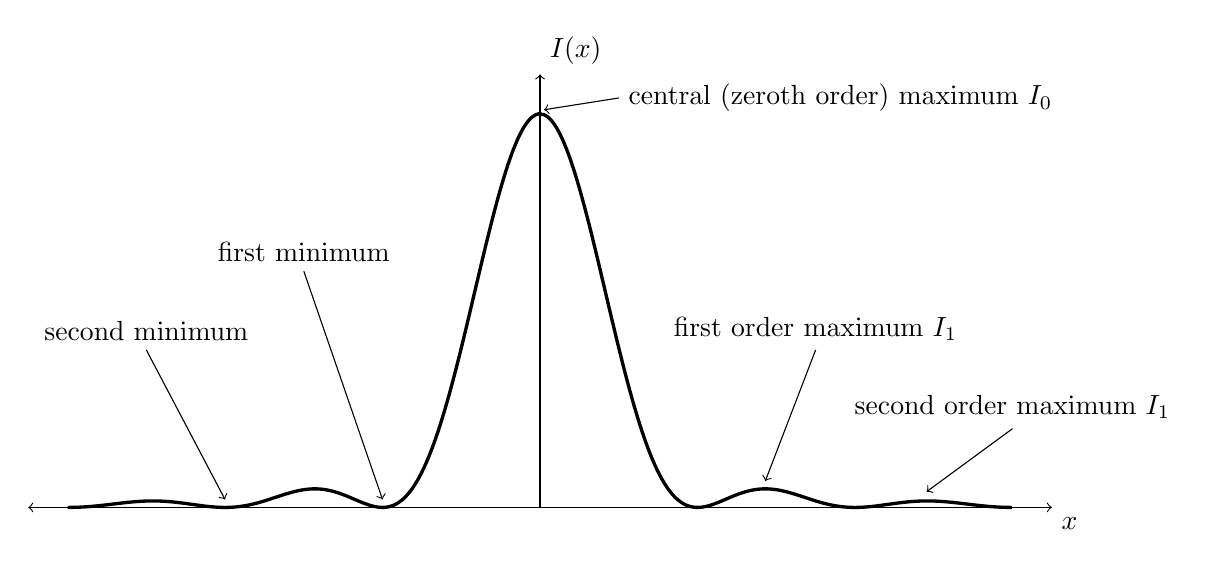
\begin{tikzpicture}
            \draw[<->] (-6.5, 0) -- (6.5, 0) node[below right, black] {$x$}; 
            \draw[->] (0, 0) -- (0, 5.5) node[above right, black] {$I(x)$} ;
        
            \draw[domain=-6:6, samples=501, very thick] plot (\x, {5*pow(sin(0.5 * pi * \x r) / (0.5 * pi * \x), 2)}); % r means in radians
            
            \draw[<-] (0.05, 5.05) -- (1, 5.2) node[right] {central (zeroth order) maximum $I_0$};
            \draw[<-] (2.86, 1/3) -- (3.5, 2) node[above] {first order maximum $I_1$};
            \draw[<-] (4.91, 1/5) -- (6, 1) node[above] {second order maximum $I_1$};
            
            \draw[<-] (-2, 1/10) -- (-3, 3) node[above] {first minimum};
            \draw[<-] (-4, 1/10) -- (-5, 2) node[above] {second minimum};
        \end{tikzpicture}
        
        \caption{The intensity profile of single-slit diffraction.}
        
        \label{fig:single-slit-diffraction-intensity}
    \end{figure}

    \begin{table}
        \centering
        
        \begin{tabular}{ c c c }
            $n$ & $y_n$ & $\sinc^2(y_n)$ \\
            \hline			
            $0$ & $0$ & $1$ \\
            $1$ & $1.4303 \, \pi$ & $0.0472$ \\
            $2$ & $2.4590 \, \pi$ & $0.0165$ \\
            $3$ & $3.4709 \, \pi$ & $0.0083$ \\
        \end{tabular}
        
        \caption{The positions $y_n$ and values of the maxima of $\sinc^2(y)$. Because $\sinc^2(0) = 1$, the last column is also the fractional (i.e., relative) intensity of the maxima relative to the center.}
        
        \label{tab:sinc-squared-maxima}
    \end{table}

    

    \section{Equipment}


    \newpage

    \section{Procedure}
    
    \subsection{Diffraction}
    
    \subsubsection{Collimating the Beam}
    For Fraunhofer diffraction, we assumed that plane waves were incident on our slits.
    To get as close to a plane wave as possible, you must use the telescope to collimate the He-Ne beam.
    Place the telescope in front of the laser (make sure you put the correct end of the telescope toward the laser).
    Adjust the height and orientation of the telescope until you can see a circular beam spot in the center of the screen (about \SI{1}{\meter} down the optical rail).
    Adjust the focus of the telescope until the beam is approximately the same diameter for the entire distance between the telescope and the screen (use a handy piece of paper to look at the beam at any point in space).
    You might also need to change the orientation of the laser to get the beam centered on the screen.
    
    \subsection{Fourier Optics}
    
    


    \newpage
    \section{Prelab Questions}
    \setcounter{subsection}{0}

    \subsection{Question 1 \hfill (1 pt.)}

    \vspace{\stretch{1}}

    \subsection{Question 2 \hfill (1 pt.)}

    \vspace{\stretch{1}}

\end{document}
